%% ------------- English version ---------------
\documentclass[english,hidelinks]{sbrt}
\usepackage{newtxtext}
\usepackage[english]{babel}
\usepackage[utf8]{inputenc}
\newtheorem{theorem}{Theorem}
%% ---------------------------------------------
\setlength{\marginparwidth}{2cm}
\usepackage{todonotes}
\newcommand\rigel[1]{\todo[color=green, inline]{\textbf{Rigel}: #1}}
\usepackage{orcidlink}
\usepackage{graphicx}
\usepackage{algorithm}
\usepackage{algpseudocode}
\usepackage{hyperref}
\usepackage[
  compatibility=false,
  font=footnotesize,
  labelsep=period,
  format=plain,
  justification=raggedright,
  singlelinecheck=false
]{caption}

\begin{document}

\title{Embedded Systems-based Predictive Maintenance for Air-Conditioning Equipment}

\author{Igor Costa, Jorge Alves, Ian Dias and Davi Ito
  \thanks{The authors are with Ibmec, Rio de Janeiro, RJ, Brazil.
  E-mails: igorcosta.silva10a@gmail.com,
  jorgedocruzeiro07@gmail.com,
  iandpcarvalho@gmail.com,
  cdavi8249@gmail.com.}%
  }

\maketitle

\markboth{XLIV BRAZILIAN SYMPOSIUM ON TELECOMMUNICATIONS AND SIGNAL PROCESSING - SBrT 2026, SEPTEMBER 29TH TO OCTOBER 2ND, 2026, SALVADOR, BA}{}

\begin{abstract}
Air-conditioning units that run around the clock in hospitals, data centers, and telecommunication shelters cannot stop for inspection, and they rarely come with a labelled failure history. This paper presents a low-cost embedded system that monitors such equipment through its vibration. An ESP32 reads a MEMS accelerometer, a current monitor, and a tachometer, and reduces each 1.23~s window to time- and frequency-domain features. A remote detector learns the healthy baseline where the machine is installed and relearns it every minute, combining an Isolation Forest with a robust distance rule. It also keeps the first baseline as a fixed reference that exposes slow drift. On three healthy sessions of a 12~V bench fan, the detector raised no false alarm in 3169 windows, while the same detector with a frozen baseline raised alarms in 5.7\% of them, and it caught all 12 abrupt faults simulated on those sessions. A drift of 1.5\% per minute entered the baseline without alarms, and the installation reference registered it as a 20\% rise.
\end{abstract}
\begin{keywords}
Predictive maintenance, air-conditioning systems, embedded systems, Internet of Things, anomaly detection.
\end{keywords}

\section{Introduction}

Embedded systems integrate dedicated computation with sensors, actuators, and communication interfaces, enabling a physical asset to be monitored and controlled close to the point where data are produced. In the Internet of Things (IoT), this combination connects physical objects to networks and analytical services: Gubbi et al. describe the convergence of wireless sensor networks, the Internet, distributed computing, and embedded sensor and actuator nodes, while Lin et al. organize IoT architectures and discuss fog/edge processing near devices to reduce latency and improve service resilience. These characteristics make embedded IoT systems suitable for continuous equipment monitoring, because measurements can be acquired at the asset, processed locally or remotely, and made available for maintenance decisions \cite{gubbi2013iot,lin2017iot}.

Predictive maintenance uses condition and operational data to support maintenance decisions before an unexpected failure, combining data acquisition, processing, health assessment, and action planning. Carvalho et al. show in a systematic review that machine-learning applications in predictive maintenance depend on the characteristics and quality of the data, as well as on the selection and validation of the method. For HVAC systems, Es-Sakali et al. review knowledge-based, physics-based, and data-driven approaches that use IoT sensors and historical measurements to assess equipment health and anticipate failures. Motivated by this context, this project focuses on air-conditioning units that operate continuously, twenty-four hours a day, in environments where cooling cannot be interrupted without affecting essential activities, such as hospital wards, data centers and server rooms, and telecommunication shelters. Continuous duty is also convenient from a measurement standpoint, because the equipment remains in a steady operating regime, which allows a stable baseline to be established and prevents daily start-stop transients from being confused with progressive degradation. The proposed prototype will investigate continuous monitoring and early anomaly detection as a first step toward predictive maintenance, without claiming remaining-useful-life estimation before a representative history of validated failures is available \cite{carvalho2019mlpdm,essakali2022hvac}.

\textit{Related work.} Yousuf et al. developed an integrated condition-monitoring and fault-detection architecture for AC induction motors. Their system combines temperature, vibration, current, voltage, and speed sensors with an Arduino-based acquisition unit, local alarms, GSM notifications, relay-based protection, and historical storage on the Blynk IoT platform. Mohammed et al. proposed a complementary Industrial IoT architecture in which a Raspberry Pi collects vibration, current, and temperature measurements and transmits them to a cloud server through MQTT. These studies demonstrate how embedded acquisition and remote communication can provide continuous evidence about motor condition, although their results still require validation before being transferred to compressors and fan motors operating under the cycling and thermal-load variations of air-conditioning systems \cite{yousuf2024iot,mohammed2023iot}.

Kolok et al. investigated whether low-cost embedded processing could support predictive-maintenance experiments on small rotating machines. Their prototype uses an ESP32 with MEMS vibration and acoustic sensors, extracts time- and frequency-domain characteristics through RMS and FFT, and applies Isolation Forest to detect deviations from healthy operation. The system achieved an overall detection accuracy above 72.9\%, showing the feasibility of lightweight local analysis but also leaving room for improvement and equipment-specific calibration. Mohammed et al. compared five supervised algorithms on an AC-motor dataset containing normal operation and induced faults, with Random Forest obtaining the highest reported accuracy. Together, these works support the evaluation of lightweight anomaly-detection and classification methods, provided that the proposed project documents its sampling procedure, fault simulation, training data, and independent test data \cite{kolok2025lowcost,mohammed2023iot}.

At the system level, predictive maintenance depends not only on the selected model, but also on the organization and quality of the complete data pipeline. Meitz et al. organized 249 publications into a framework of nine categories and 73 attributes, covering condition monitoring, fault detection, degradation modeling, scheduling, data handling, prognostic techniques, and evaluation. Gupta et al. complemented this broad view with a field study of airport baggage-handling conveyors, where vibration data were collected from a live system despite the absence of historical run-to-failure records. Their pipeline distinguished anomalies from noisy observations, processed heterogeneous maintenance records, and compared four classifiers. Random Forest achieved the best reported motor--gearbox classification performance, with precision, recall, and F1-score of 0.86. These findings indicate that sensing, cleaning, labeling, and evaluation should be treated as connected parts of the proposed system rather than as isolated modeling tasks \cite{meitz2025pdmframework,gupta2023baggage}.

Beyond detecting that something deviates from normal operation, a maintenance system must indicate what deviated, so that the alert can be acted upon. Tormos et al. addressed this problem in air-conditioning units of urban bus fleets, where operational data are collected continuously but are rarely accompanied by reliable fault labels. The authors first map the available measurements onto the vapor-compression refrigeration cycle, which yields physically meaningful features and an operational baseline. An Isolation Forest then identifies deviations from that baseline, and Kernel SHAP attributes each deviation score to the variables that produced it, with the attributions grouped into physics-informed explanation families so that anomalies are read as refrigeration mechanisms rather than as isolated variables. The reported results distinguish physically plausible rare operating states, inspection candidates, and ambiguous cases without relying on confirmed fault labels. The study is based on bus fleet telematics rather than on stationary equipment, and the attribution step is computationally heavy for a microcontroller, which places it on the server side of the proposed architecture. It nevertheless supports two decisions of this project: learning the healthy baseline instead of requiring labelled failures, and reporting which measurement triggered each alert \cite{tormos2026hvacxai}.

The implementation, documentation, and experimental material produced in this project are publicly available in the project repository \cite{repo}.

This work proposes an embedded system that monitors the condition of air-conditioning units under uninterrupted duty and flags anomalies early. The prototype reads vibration at the equipment through a low-cost microcontroller, records electrical current and fan speed alongside it, and computes time- and frequency-domain features on the spot. The measurements then reach a remote application, which compares them against the healthy operating baseline and reports what deviated. Four aspects of this design are our contribution. The architecture pairs local acquisition and lightweight edge processing with remote communication, sized for equipment that stays in a steady regime and cannot have its cooling interrupted. The detection strategy learns the healthy baseline instead of requiring a labelled failure history, which is the realistic condition for equipment that has never been instrumented, and follows what Tormos et al. and Gupta et al. report from field deployments with the same absence of run-to-failure records \cite{tormos2026hvacxai,gupta2023baggage}. The system names the measurement that produced the alert, so the maintenance team gets something to act on instead of an undifferentiated warning. And the evaluation injects faults of known size and timing into independent recordings of healthy operation, so every alarm can be checked against what was done. We restrict the prototype to the condition monitoring, data handling, fault detection, and evaluation stages of the framework organized by Meitz et al. Degradation modelling, prognostics, and remaining-useful-life estimation stay out, because they need a representative history of validated failures that the prototype does not have \cite{meitz2025pdmframework}. The initial tests run on a bench built around a 12~V fan, the same class of machine as the condenser fan of an air-conditioning unit, which lets faults be induced in a controlled way. A bench fan is still not a compressor, so the results characterise the method rather than validate it on a real unit.

The rest of this work is organized as follows. Section~\ref{sec:system-description} describes the system under development, its sensors, microcontroller and communication protocol, together with the configuration defined for the first experiments. Section~\ref{sec:method} details the proposed method, covering signal acquisition, feature extraction, the operating baseline, the detection of deviations and the interpretation of each alert. We then report the results obtained with the prototype in Section~\ref{sec:results}, and Section~\ref{sec:conclusion} concludes the work, compares the proposed method with an alternative solution and outlines the next steps.

\section{System Description}
\label{sec:system-description}

The monitoring station is built around a single low-cost microcontroller that reads the sensors at the equipment, computes features locally, and sends the result onward. Kolok et al. showed that a board of this class can extract time- and frequency-domain characteristics and run a lightweight anomaly detector without a server, and Lin et al. describe why processing near the device reduces latency and keeps the service running when the link does not \cite{kolok2025lowcost,lin2017iot}. The prototype uses an ESP32 module, which combines integrated Wi-Fi with enough memory to compute the RMS and the frequency transform on the board itself, so neither an external radio nor a server is required for the processing.

\subsection{Vibration Sensing}

Vibration is the main signal of the system, and the anomaly detector is trained on its features alone. A MEMS accelerometer is fixed to the shell of the rotating component and reports acceleration along three axes. For each axis and each window, the firmware computes the RMS, the peak, the kurtosis, and a discrete Fourier transform from which it keeps the dominant frequency and its amplitude. RMS and the Fourier transform are the same pair of characteristics that Kolok et al. applied to small rotating machines, and Yousuf et al. combine with electrical measurements on induction motors \cite{kolok2025lowcost,yousuf2024iot}. Mechanical coupling decides whether the reading means anything: a sensor that is not rigidly attached measures its own movement rather than the machine. On the bench it is bonded to the side of the fan frame. On an air conditioner it is held to the compressor shell by a magnetic base or structural adhesive.

\subsection{Electrical Current Sensing}

A motor under friction draws more current to hold its speed. Yousuf et al. and Mohammed et al. both include current among the quantities they acquire from motors under induced faults \cite{yousuf2024iot,mohammed2023iot}.

The prototype uses two different sensors for this single quantity. On the bench, where the machine runs at low voltage, a shunt monitor on the supply line measures the current directly. On an air-conditioning unit, where the compressor runs from the mains, a split-core current transformer clamps around one conductor and measures by induction, without cutting any wire and without contact with the supply. The distinction matters for safety as much as for accuracy, and it is declared here because the two setups are not interchangeable.

\subsection{Processing and Communication}

The microcontroller acquires vibration, current, and fan speed and computes the window features. In a field installation it publishes each window through MQTT, a lightweight publish and subscribe protocol for low-bandwidth and intermittent links. Mohammed et al. adopt the same arrangement, with an embedded acquisition unit transmitting vibration, current, and temperature to a remote server, and Gubbi et al. describe the wider architecture in which such devices deliver data to analytical services \cite{mohammed2023iot,gubbi2013iot}. The prototype sends the windows to a laptop over the USB serial link instead. The campus network admits a device only after a login on a web page, which the microcontroller cannot complete, so MQTT is left for the field installation. The receiving side compares each window against the healthy baseline and reports which measurement produced the alert. Only the vibration features feed the detector. Current and speed are kept for inspection.

\subsection{Experimental Configuration}

The first experiments run on a bench built around a 12~V fan supplied at a fixed voltage and bonded upright to a wooden base, with the accelerometer bonded to the side of the fan frame and the shunt monitor in series with the supply. The fan exposes a tachometer output, which adds rotational speed at no extra cost.

The evaluation reported here uses three independent sessions of healthy operation, recorded on different occasions with the fan starting from rest. They last 12.3, 21.5, and 37.1 minutes, or 600, 1050, and 1816 windows. Faults are injected by software into those recordings, as a change of known size applied to known windows, so every alarm can be checked against what was done. Physical disturbances enter only in live tests on the bench, where the fan is shaken by hand or its frame is flicked, and those tests are reported qualitatively.

Imbalance, friction, and obstruction runs, each recorded apart from the others, belong to the next stage of the project, when the detector will also be asked to name the mechanism behind an alarm. Gupta et al. report that slicing training and test data from a single acquisition inflates the measured performance, and Meitz et al. treat evaluation as a stage of its own rather than an afterthought \cite{gupta2023baggage,meitz2025pdmframework}. The same rule holds here: every evaluation run learns its baseline from the first two minutes of that run and is scored only on the windows that follow.

\section{The Method}
\label{sec:method}

\begin{figure*}[t]
  \centering
  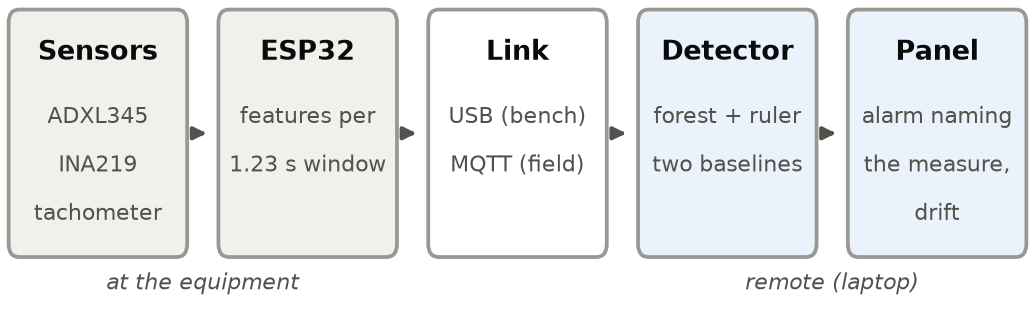
\includegraphics[width=\textwidth]{assets/arquitetura.png}
  \caption{Architecture of the prototype. The ESP32 reduces each window to features at the equipment, and a remote application learns the healthy baseline of that installation and reports deviations from it.}
  \label{fig:architecture}
\end{figure*}

% Foto do prototipo: suba a foto no Overleaf como assets/prototipo.jpg e
% descomente o bloco abaixo.
% \begin{figure}[t]
%   \centering
%   \includegraphics[width=\columnwidth]{assets/prototipo.jpg}
%   \caption{Bench prototype: 12~V fan bonded upright to a wooden base, ADXL345 bonded to the fan frame, INA219 in series with the supply, and ESP32 connected to a laptop over USB.}
%   \label{fig:prototype}
% \end{figure}

Fig.~\ref{fig:architecture} shows the processing chain. The ESP32 reads the sensors and reduces each window to a few numbers, and a remote application learns what normal operation looks like at that installation and flags what departs from it. The subsections below follow the chain from the sensor to the alert, and Algorithm~\ref{alg:detector} summarizes the detector.

\subsection{Acquisition and Features}

The accelerometer samples at a nominal 400~Hz into its internal 32-sample FIFO buffer in stream mode, and the ESP32 drains the buffer over I2C at 100~kHz. Each window holds 512 samples. The firmware estimates the actual sample rate from the duration of every window instead of assuming the nominal one. It does not yet count FIFO overflows, so the continuity of the samples inside a window remains to be verified. On the bench it measured 417~Hz, which gives windows of 1.23~s and a frequency resolution of 0.81~Hz. For each axis, the firmware removes the mean and computes the RMS, the peak absolute value, and the kurtosis. It then applies a Hann window and a 512-point FFT and keeps the largest spectral peak and its frequency. The shunt monitor is averaged over the window, and an interrupt counts the tachometer pulses with a 4~ms debounce. Each window leaves the board as one line of 22 comma-separated fields.

The per-axis values depend on how the sensor sits on the machine. In early sessions, the fan shifted slightly on its base and moved vibration energy from one axis to another while the total stayed the same. The detector therefore works on five quantities that do not depend on orientation: the vector sums of the three RMS values, of the three peaks, and of the three spectral peak amplitudes, the mean kurtosis of the three axes, and their median dominant frequency. Current and speed stay out of the detector and are recorded for inspection.

\subsection{Detection}

Each window passes two tests, and either one raises an alarm. The first is an Isolation Forest, the detector that Kolok et al. and Tormos et al. applied to healthy baselines \cite{kolok2025lowcost,tormos2026hvacxai}. It is trained with 150 trees on the standardized totals of the healthy windows, and its threshold is the 0.2\% quantile of the training scores. The forest judges whether the combination of the five totals resembles the baseline, but its score saturates far from it. In early tests, a vibration 30\% stronger than normal stayed close to the threshold.

The second test, which we call the ruler, measures how far each total sits from the baseline in robust units,
\begin{equation}
  z = \frac{x - \tilde{x}}{s}, \qquad s = \max\left(1.4826\,\mathrm{MAD},\; 0.03\,\tilde{x}\right),
\end{equation}
where $\tilde{x}$ is the median of the total over the healthy windows and MAD is their median absolute deviation. The ruler raises an alarm when the RMS, the peak, or the spectral peak amplitude reaches $|z| > 6$. The median and the MAD keep a few seconds of start-up shocks from shifting the baseline, and the 3\% floor stops a very quiet baseline from making small changes look large.

Live tests showed the forest flagging isolated windows whose totals sat only 1.7 to 2.8 deviations from the median, the size of ordinary noise. The forest now raises an alarm only when it flags two windows in a row and at least one total reaches $|z| \geq 3$. Each alarm names the total that moved the most, as a number of deviations or, beyond 20 deviations, as a multiple of its normal value. This plays the role that SHAP attribution plays in the work of Tormos et al., reduced to what a distance per measurement can explain \cite{tormos2026hvacxai}.

\subsection{Adaptive Baseline and Installation Reference}

A model trained once describes the conditions of the day it was trained. On the bench, the same fan vibrated at about 0.15~g on one table and 0.10~g on another, a larger difference than the one produced by blocking its air inlet, and the vibration kept drifting slowly for more than 20 minutes while the motor warmed up. A fixed baseline would read either change as a fault. The detector therefore learns the healthy baseline where it is installed, during its first two minutes of operation, and relearns it every minute from the last ten minutes of windows that raised no alarm. A slow change, such as warming or the temperature of the day, enters the baseline. A fast one, such as a blocked inlet, becomes an alarm. Kolok et al. list adaptive thresholds among the open questions of their ESP32 detector when load and speed change, which is the situation this design addresses \cite{kolok2025lowcost}.

Relearning also gives the fault a way into the baseline, and three rules keep it out. A window that raised an alarm never enters the baseline, and neither do the windows of the 30~s that follow it. The last 30~s before each update stay out, so the first windows of a fault, which may not have crossed the threshold yet, are not learned. The first 15~s of the initial learning are discarded because they hold the motor start-up.

An adaptive baseline carries a risk of its own: it can grow used to a fault that develops slowly. A mounting screw that loosens a little each day looks almost normal when compared with the day before, and the detector would keep absorbing it. To keep that kind of change visible, the detector stores the baseline learned at installation and never updates it. The panel reports the drift, the relative difference between the median vibration of the current baseline and that installation reference. Environmental changes come and go, with the afternoon warmer than the night and the next morning close to the start again. Wear only moves in one direction. A drift that keeps growing over days without returning points to a slow change that the adaptive baseline alone would hide. A fault that persists is not absorbed either: when alarms cover at least 80\% of the windows for three minutes, the detector asks for an inspection and keeps its baseline until the alarms stop.

In the prototype, the drift is shown to the operator but does not yet trigger an alarm. Telling weather apart from wear with confidence needs days of recording and the operating context that explains the load, namely current, speed, and ambient temperature, so it is left for the next stage of the project.

\begin{algorithm}[t]
\caption{Adaptive detector, run for every window}
\label{alg:detector}
\begin{algorithmic}[1]
\State $x \gets$ the five totals of the window
\If{the detector is still learning (first 120~s)}
  \State store $x$, skipping the first 15~s
  \State at 120~s, train forest and ruler; reference $r_0 \gets \tilde{x}_{\mathrm{RMS}}$
\Else
  \State $z \gets (x - \tilde{x}) / s$
  \State $a_{\mathrm{r}} \gets |z| > 6$ for RMS, peak, or spectral peak
  \State $a_{\mathrm{f}} \gets$ forest flags this and the previous window and $\max |z| \geq 3$
  \If{$a_{\mathrm{r}}$ or $a_{\mathrm{f}}$}
    \State report the total with the largest $|z|$
    \State block learning for 30~s
  \EndIf
  \If{alarms cover $\geq 80\%$ of the last 180~s}
    \State request an inspection
  \EndIf
  \State store $x$, marked learnable if no alarm and not blocked
  \If{60~s since the last update and not blocked}
    \State retrain on learnable windows from $t-600$~s to $t-30$~s
  \EndIf
  \State drift $\gets \tilde{x}_{\mathrm{RMS}} / r_0 - 1$
\EndIf
\end{algorithmic}
\end{algorithm}

\section{Results}
\label{sec:results}

\subsection{Bench Behaviour}

The bench delivered stable windows across the three sessions. The sample rate stayed at 417~Hz, the median total RMS was 0.150, 0.155, and 0.144~g, and the dominant frequency sat between 46.3 and 46.5~Hz, which corresponds to about 2780~rpm. The fan drew between 148 and 153~mA. The vibration was not stationary within a session. In the first two sessions it rose about 7\% over the first ten minutes, and in the third it fell 8\% over the same interval and 11\% by the end. A drift of this size is comparable to the faults the system has to find, and it is the reason for the adaptive baseline.

The tachometer did not hold up. It reported between 3490 and 4230~rpm, 25\% to 52\% above the speed given by the vibration peak, and its error changed from one session to the next. Electrical noise on the pulse line is the likely cause. A pulse-width filter removed the readings altogether, so the speed comes from the vibration spectrum until the tachometer circuit is fixed.

\subsection{False Alarms on Healthy Operation}

Table~\ref{tab:false-alarms} counts the alarms raised on the healthy sessions after the two minutes of learning. The adaptive detector raised none in 3169 windows. The same detector with its baseline frozen after the first two minutes, which is how a model trained once behaves, raised alarms in 5.7\% of the windows. Almost all of them came from the third session, where the vibration drifted away from the level learned at its start.

\begin{table}[t]
\caption{Windows in alarm on the healthy sessions, after learning.}
\label{tab:false-alarms}
\centering
\begin{tabular}{lccc}
\hline
Session & Windows & Adaptive & Frozen baseline \\
\hline
1 (12.3 min) & 501 & 0 & 2 (0.4\%) \\
2 (21.5 min) & 951 & 0 & 0 \\
3 (37.1 min) & 1717 & 0 & 180 (10.5\%) \\
\hline
Total & 3169 & 0 & 182 (5.7\%) \\
\hline
\end{tabular}
\end{table}

\subsection{Abrupt Fault}

An abrupt fault was simulated by raising the RMS, the peak, and the spectral peak amplitude of every axis by 30\% for 60~s. It was injected every five minutes along each session, starting at minute five, one fault per run, for 12 runs. The detector caught all 12 faults, and 584 of the 585 windows inside them (99.8\%) raised an alarm. No run led to an inspection request, since every fault ended before three minutes.

The two tests did not contribute equally. The ruler flagged 98.6\% of the fault windows, alone in 45.1\% and together with the forest in 53.5\%, and the forest alone added 1.2\%. For a change that scales the amplitude, the ruler carries the detection and the forest confirms it. The forest stays in the detector because it judges the five totals together, which matters for a fault that moves the kurtosis or the frequency without changing the amplitude. The simulated fault does not test that case.

\subsection{Slow Drift}

A slow fault was simulated on the last 27 minutes of the third session, after its initial decline. From minute four on, the amplitudes rose linearly at 1.0, 1.5, and 2.0\% per minute. Table~\ref{tab:drift} and Fig.~\ref{fig:drift} show the result.

\begin{table}[t]
\caption{Slow drift simulated on session 3: windows in alarm during the rise, drift against the installation reference at the end, and inspection request.}
\label{tab:drift}
\centering
\begin{tabular}{lcccc}
\hline
Rate & Adaptive & Frozen & Final drift & Inspection \\
\hline
1.0\%/min & 2.8\% & 15.5\% & +12.2\% & no \\
1.5\%/min & 4.5\% & 44.0\% & +20.0\% & no \\
2.0\%/min & 63.1\% & 57.2\% & +1.1\% & after 11.8 min \\
\hline
\end{tabular}
\end{table}

\begin{figure}[t]
  \centering
  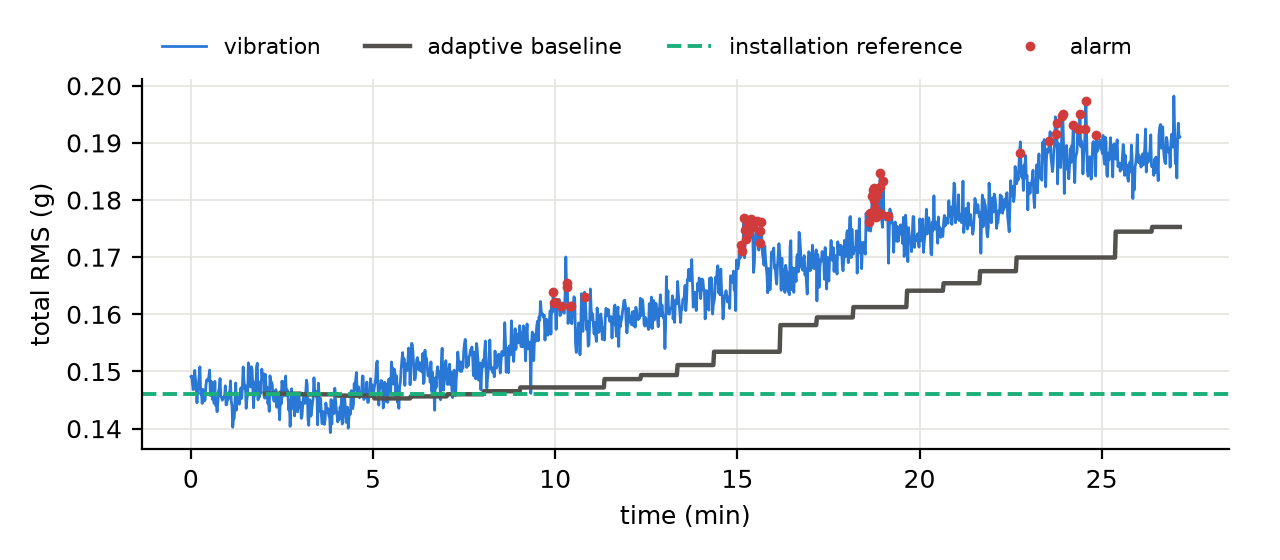
\includegraphics[width=\columnwidth]{results/avaliacao_lenta.png}
  \caption{Slow drift of 1.5\% per minute, starting at minute four. The adaptive baseline follows the vibration with few alarms, and the gap to the installation reference records the change.}
  \label{fig:drift}
\end{figure}

Up to 1.5\% per minute, the adaptive baseline followed the change with few alarms, while the frozen baseline raised alarms in up to 44\% of the windows. Following the change is the intended behaviour for warming and weather, and it is also the risk: at the end of the 1.5\% run the baseline had moved 20\% above the installation, and only the drift showed it. At 2\% per minute the baseline could no longer keep up. The alarms blocked the updates and the baseline stayed near the installation value, which is why the final drift reads only +1.1\%, and after 11.8 minutes of rising vibration the detector requested an inspection. For this configuration, the boundary between absorbing a change and treating it as a fault lies between 1.5 and 2\% per minute, set by the update period, the ten-minute memory, and the width of the ruler. Wear on a real unit develops over days, far below either rate, so it would enter the baseline and show only in the drift. That is why the drift, and not the alarm, is the channel meant for slow wear.

\subsection{Live Tests}

The detector also ran live on the bench, fed by the serial link. Shaking the fan by hand and flicking its frame raised alarms during the disturbance, and the panel named the measurement that moved. These runs also exposed the false alarms of the forest on ordinary noise described in Section~\ref{sec:method}, which led to the two-window and three-deviation conditions.

\section{Conclusion}
\label{sec:conclusion}

This work presented a low-cost embedded system for the condition monitoring of air-conditioning equipment in continuous duty. An ESP32 reduces the vibration of the machine to per-window features, and a remote detector learns the healthy baseline where the machine is installed, relearns it every minute, and keeps the installation baseline as a fixed reference. On three healthy sessions of a bench fan, the detector raised no false alarm in 3169 windows and caught all 12 abrupt faults simulated on those sessions.

The alternative solution is the approach of Kolok et al., a detector trained once on healthy operation and then kept fixed \cite{kolok2025lowcost}. On the same data, freezing the baseline raised alarms in 5.7\% of the healthy windows and in up to 44\% of the windows of a slow drift that the adaptive baseline absorbed. The adaptive baseline pays for this with a blind spot: a change slower than about 1.5\% per minute enters the baseline, and only the drift against the installation reference reveals it.

The results have clear limits. The faults were simulated by software on recordings of a single fan, a bench fan is not a compressor, the recordings cover minutes rather than days, and the tachometer still needs repair. The next steps follow from these limits: recording imbalance, friction, and obstruction in separate runs and naming the mechanism behind each alarm, fixing the tachometer, publishing the windows over MQTT on a network that does not require a web login, and turning the drift into an alert once days of recordings and the operating context, namely current, speed, and ambient temperature, can separate weather from wear.

\bibliographystyle{ieeetr}
\bibliography{refs}

\end{document}
